\refstepcounter{Exercise}
\clearpage\subsection*{\theExercise クエリストリングを使ってLEDを操作する}
\addtocounter{Exercise}{-1}\refstepcounter{Exercise}\label{E:QS}

% \clearpage\subsection*{クエリストリングを使ってLEDを操作する}
この例では、クエリストリングを使ってLEDを点灯消灯させてみましょう。


\bigskip

まずは、ブラウザを開いて、

localhost:3000/cgi-bin/qsled.hsp?led=17\&val=1

を入力してみましょう。

%
%ぶらうざで開いた開いた画面
%koyaman
%September 20, 2019 2:50 AM


\centering
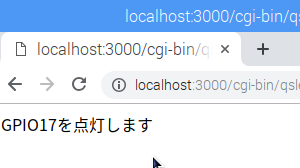
\includegraphics[width=0.8\textwidth]{text07-img/ome7-img055.png}
\flushleft

実行するとLED17が光ります。val=1をval=0にすると消えます。URLに埋め込まれた情報をもとにCGIプログラムはLEDを操作していることがわかります。URLに埋め込まれた情報はクエリストリングと呼ばれます。


\bigskip

クエリストリングを\ruby{詳}{くわ}しく見てみましょう。

クエリストリングとはURLの最後に?をつけて始めます。?のあとには

名前(変数名みたいなもの) = 値

の形を続けます。例えば、

localhost:3000/cgi-bin/qsled.hsp?led=17

のようにかけます。この場合は、

名前がled、値が17となります。

複数の情報を渡したい場合は\&を使います。

localhost:3000/cgi-bin/qsled.hsp?led=17\&val=1

のようになります。

名前1がled、値1が17となり

名前2がval、値2が1となります。

このクエリストリングをプログラムから扱う方法を次に学びましょう。

\clearpage
プログラム解説






\begin{table}[htbp]
    \centering
    % \caption{文字タイプ表}
    \begin{tabular}{|l|}
        \hline
        
        1. \#include {\textquotedbl}hsp3cl.as{\textquotedbl}\\ 
        2. \#include {\textquotedbl}rpz-gpio-cl.as{\textquotedbl}\\
        3. \#include {\textquotedbl}cgi.as{\textquotedbl}\\
        4. mes {\textquotedbl}Content-type: text/html{\textbackslash}n{\textquotedbl}\\
        5. mes {\textquotedbl}{\textless}html{\textgreater}{\textless}head{\textgreater}{\textless}meta charset={\textbackslash}{\textquotedbl}utf-8{\textbackslash}{\textquotedbl}{\textgreater}{\textless}/head{\textgreater}{\textless}body{\textgreater}{\textquotedbl}\\
        6. ; クエリストリングからledを探して、値をled\_portへ入れる\\
        7. getqueryval {\textquotedbl}led{\textquotedbl}, led\_port\\
        8. ; クエリストリングからvalを探して、値をled\_valへ入れる\\
        9. getqueryval {\textquotedbl}val{\textquotedbl}, led\_val\\
        10. ;文字列なので数値へ変換する\\
        11. led\_port = int(led\_port)\\
        12. led\_val = int(led\_val)\\
        13. \\
        14. ; 点灯消灯を判断して、メッセージをpタグで表示する\\
        15. if(led\_val = 1) \{ \\
        16. \ \ \ \ mes {\textquotedbl}{\textless}p{\textgreater}GPIO{\textquotedbl} + led\_port + {\textquotedbl}を点灯します{\textless}/p{\textgreater}{\textquotedbl}\\
        17. \} else \{ \\
        18. \ \ \ \ mes {\textquotedbl}{\textless}p{\textgreater}GPIO{\textquotedbl} + led\_port + {\textquotedbl}を消灯します{\textless}/p{\textgreater}{\textquotedbl}\\ 
        19. \}\\
        20. \\
        21. ;クエリストリングのledで指定されたGPIOにvalで指定された値を書き込む\\
        22. ; localhost:3000/cgi-bin/qsled.hsp?led=17\&val=1\\
        23. ; の場合、LED17を点灯させる\\
        24. cgpio led\_port, led\_val\\
        25. mes {\textquotedbl}{\textless}/body{\textgreater}{\textless}/html{\textgreater}{\textquotedbl}\\
        26. end\\
        
        \hline
    \end{tabular}
\end{table}


\bigskip



\bigskip


\bigskip

7行目、9行目で使用している

getqueryval命令でクエリストリングを受け取ります。この命令は

getqueryval 名前, 値を入れる変数

のように使います。クエリストリングから名前を探して、変数へ値を文字列としていれます。

例えば、

getqueryval led, led\_port

の場合にlocalhost:3000/cgi-bin/qsled.hsp?led=17

とクエリストリングを与えたとすると、

led\_portには17が入ります。

11,12行目で

文字列から数値へ変換しています。

15〜19行目では、点灯するのか消灯するのかを条件判断を使って判断しています。led\_valが1のとき(val=1がクエリストリングで与えられたとき)に点灯する、その他のときは消灯するとします。

24行目で実際に点灯、消灯を行います。

cgpio命令は数値でGPIO番号、オンオフ(1,0)を受け付けるので、文字列から変換をしました。


\bigskip

\refstepcounter{Question}\theQuestion

{\bfseries

GPIO17以外のLEDを光らせてみよう。}


\bigskip


\bigskip